%%%%%%%%%%%%%%%%%%%%%%%%%%%%%%%%%%%%%%%%%%%%%%%%%%%%%%%%%%%%%%%%%%%%%%%%%%%%%%%
\section{Aberration Measurement and Correction}
%%%%%%%%%%%%%%%%%%%%%%%%%%%%%%%%%%%%%%%%%%%%%%%%%%%%%%%%%%%%%%%%%%%%%%%%%%%%%%%

%explain what are abberations, how they arrise, why it is good to correct them

%here is some stuff that I collected/copied from the paper you gave me

For the purpose of understanding the operation of an adaptive optical system, it is best to think of aberrations in terms of distortions of an optical wavefront.

\begin{figure}[tbh]
        \centering
        \begin{subfigure}[b]{0.4\textwidth}
                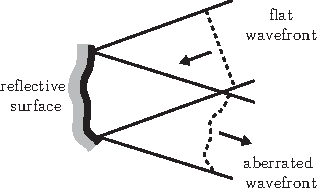
\includegraphics[width=\textwidth]{images/wavefront_distortions_reflection}
                \caption{Reflection.}
                \label{fig:abberation_reflection}
        \end{subfigure}
				\hspace{1em}
        \begin{subfigure}[b]{0.3\textwidth}
                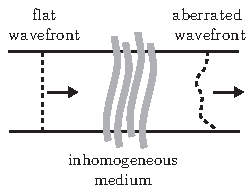
\includegraphics[width=\textwidth]{images/wavefront_distortions_transmission}
                \caption{Transmission.}
                \label{fig:abberation_trans}
        \end{subfigure}
        \caption{Wavefront aberrations due to (a) reflection from a non planar surface and (b)  caused by propagation through a non-uniform refractive index distribution. Image after~\cite{Aberrations_book}.}
\label{fig:abberations}
\end{figure} 

Representing aberrations in this way can simplify the design, control and characterisation of adaptive optics. The choice of modes for a particular application is often influenced by some aspect of the system, such as the deformation modes of a deformable mirror or the statistics of the induced aberrations. Otherwise, the modal representation may be chosen through mathematical convenience. For example, Zernike polynomials are often used for systems with circular apertures as they form a complete, orthogonal set of functions defined over a unit circle

As with all optical systems, microscopes can also suffer from aberrations due to imperfections in the optical components. In practice, no system can be totally free from aberrations and so systems are designed to maintain aberrations below a particular tolerance for a given set of imaging conditions, such as wavelength, magnification and field of view. Significant aberrations can be introduced if a microscope is used outside its design specifications, for example at the incorrect wavelength or at a difierent temperature (see Chapter 11 of Ref. 9).


%%%%%%%%%%%%%%%%%%%%%%%%%%%%%%%%%%%%%%%%%%%%%%%%%%%%%%%%%%%%%%%%%%%%%%%%%%%%%%%
\subsection{Wavefront Sensing}
\label{sec:WavefrontSensing}

%------------------------------------------------------------------------------
\subsubsection{Interferometry}
\label{sec:DirectWavefrontSensing_interferometry}
%not sure if this is used for microscopy, we should at least mention it

%------------------------------------------------------------------------------
\subsubsection{Shack-Hartman Wavefront Sensor}
\label{sec:DirectWavefrontSensing_SHWS}

%------------------------------------------------------------------------------
\subsubsection{Indirect Wavefront Sensing}
\label{sec:IndirectWavefrontSensing}

%%%%%%%%%%%%%%%%%%%%%%%%%%%%%%%%%%%%%%%%%%%%%%%%%%%%%%%%%%%%%%%%%%%%%%%%%%%%%%%
\subsection{Aberration Correction}
\label{sec:AberrationCorrection}
% just mention the basic principles, i.e. liquid crystal, deformable mirror, computational

%------------------------------------------------------------------------------
\subsection{Deformable Mirror }
\label{sec:DeformableMirror}

%------------------------------------------------------------------------------
\subsubsection{Liquid Crystal Spatial Light Modulators}
\label{sec:LiquidCrystalSpatialLightModulators}
% I used Nematic Liquid Crystalls for my Bachelor Thesis, so if you need 
% infos or graphs about them, let me know and I might be able to help

%%%%%%%%%%%%%%%%%%%%%%%%%%%%%%%%%%%%%%%%%%%%%%%%%%%%%%%%%%%%%%%%%%%%%%%%%%%%%%%
\subsection{Control Strategies}
\label{sec:ControlStrategies}
